\documentclass[12pt]{article}
\usepackage{tikz}
\usepackage[utf8]{inputenc}

\begin{document}

\begin{figure}
\center
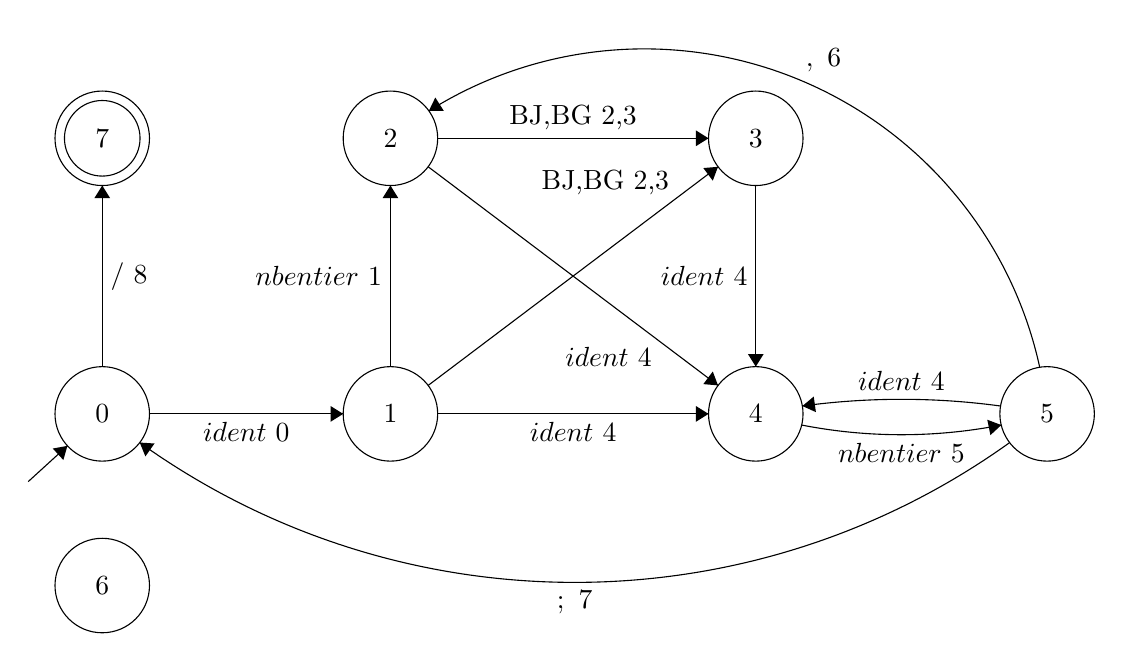
\begin{tikzpicture}[scale=0.2]
\tikzstyle{every node}+=[inner sep=0pt]
\draw [black] (11.1,-33.3) circle (3);
\draw (11.1,-33.3) node {$0$};
\draw [black] (29.4,-33.3) circle (3);
\draw (29.4,-33.3) node {$1$};
\draw [black] (29.4,-15.8) circle (3);
\draw (29.4,-15.8) node {$2$};
\draw [black] (52.6,-15.8) circle (3);
\draw (52.6,-15.8) node {$3$};
\draw [black] (52.6,-33.3) circle (3);
\draw (52.6,-33.3) node {$4$};
\draw [black] (71.1,-33.3) circle (3);
\draw (71.1,-33.3) node {$5$};
\draw [black] (11.1,-15.8) circle (3);
\draw (11.1,-15.8) node {$7$};
\draw [black] (11.1,-15.8) circle (2.4);
\draw [black] (11.1,-44.2) circle (3);
\draw (11.1,-44.2) node {$6$};
\draw [black] (14.1,-33.3) -- (26.4,-33.3);
\fill [black] (26.4,-33.3) -- (25.6,-32.8) -- (25.6,-33.8);
\draw (20.25,-33.8) node [below] {$ident\mbox{ }0$};
\draw [black] (11.1,-30.3) -- (11.1,-18.8);
\fill [black] (11.1,-18.8) -- (10.6,-19.6) -- (11.6,-19.6);
\draw (11.6,-24.55) node [right] {$/\mbox{ }8$};
\draw [black] (29.4,-30.3) -- (29.4,-18.8);
\fill [black] (29.4,-18.8) -- (28.9,-19.6) -- (29.9,-19.6);
\draw (28.9,-24.55) node [left] {$nbentier\mbox{ }1$};
\draw [black] (32.4,-15.8) -- (49.6,-15.8);
\fill [black] (49.6,-15.8) -- (48.8,-15.3) -- (48.8,-16.3);
\draw (41,-15.3) node [above] {BJ,BG 2,3};
\draw [black] (31.8,-31.49) -- (50.2,-17.61);
\fill [black] (50.2,-17.61) -- (49.27,-17.69) -- (49.87,-18.49);
\draw (43.05,-19.45) node [above] {BJ,BG 2,3};
\draw [black] (32.4,-33.3) -- (49.6,-33.3);
\fill [black] (49.6,-33.3) -- (48.8,-32.8) -- (48.8,-33.8);
\draw (41,-33.8) node [below] {$ident\mbox{ }4$};
\draw [black] (31.8,-17.61) -- (50.2,-31.49);
\fill [black] (50.2,-31.49) -- (49.87,-30.61) -- (49.27,-31.41);
\draw (43.25,-29.05) node [below] {$ident\mbox{ }4$};
\draw [black] (52.6,-18.8) -- (52.6,-30.3);
\fill [black] (52.6,-30.3) -- (53.1,-29.5) -- (52.1,-29.5);
\draw (52.1,-24.55) node [left] {$ident\mbox{ }4$};
\draw [black] (68.186,-34.009) arc (-78.92391:-101.07609:32.981);
\fill [black] (68.19,-34.01) -- (67.3,-33.67) -- (67.5,-34.65);
\draw (61.85,-35.12) node [below] {$nbentier\mbox{ }5$};
\draw [black] (6.4,-37.6) -- (8.89,-35.33);
\fill [black] (8.89,-35.33) -- (7.96,-35.5) -- (8.63,-36.23);
\draw [black] (55.558,-32.8) arc (97.74772:82.25228:46.676);
\fill [black] (55.56,-32.8) -- (56.42,-33.19) -- (56.28,-32.2);
\draw (61.85,-31.87) node [above] {$ident\mbox{ }4$};
\draw [black] (31.842,-14.06) arc (122.13361:12.33429:25.709);
\fill [black] (31.84,-14.06) -- (32.79,-14.06) -- (32.25,-13.21);
\draw (56.91,-11.6) node [above] {$,\mbox{ }6$};
\draw [black] (68.719,-35.124) arc (-54.36133:-125.63867:47.4);
\fill [black] (13.48,-35.12) -- (13.84,-36) -- (14.42,-35.18);
\draw (41.1,-44.5) node [below] {$;\mbox{ }7$};
\end{tikzpicture}
\caption{Automate d'analyse syntaxique des fiches de livraison viticole. Les arcs sont étiquetés par les items lexicaux suivis des numéros d'actions.}
\end{figure}

\end{document}
